\documentclass{beamer}
\usepackage[export]{adjustbox}
\usepackage{booktabs}
\usepackage{caption}
\usepackage{fancyvrb}
\usepackage{graphicx}
\usepackage{mathtools}
\usepackage{pdfpages}
\usepackage{siunitx}
\usepackage{tikz}
\usetikzlibrary{positioning}
\usepackage{xcolor}
\usepackage{xspace}

\setbeamertemplate{navigation symbols}{} %turn off navigation symbols

\makeatother
\setbeamertemplate{footline}
{
	\leavevmode%
	\hbox{%
		\begin{beamercolorbox}[wd=0.3\paperwidth,left]{white}
			\usebeamerfont{author in head/foot}\insertshortauthor
		\end{beamercolorbox}
    	\begin{beamercolorbox}[wd=0.4\paperwidth,center]{white}
    		\usebeamerfont{title in head/foot}\textbf{\insertshorttitle: \insertshortsubtitle}
    	\end{beamercolorbox}
    	\begin{beamercolorbox}[wd=0.3\paperwidth,right]{white}
    		\insertframenumber{} / \inserttotalframenumber
    	\end{beamercolorbox}
    }%
  	\vskip0pt%
}
\makeatletter
%\setbeamertemplate{footline}[frame number]


\title{Summer oscillation analysis}
\subtitle{Event rate validation}

\author{\textbf{Chris Barry}, Andy Chappell}
\institute{     
\includegraphics[height=1.2cm]{images/t2k_logo_medium}\\
\includegraphics[width=0.3\textwidth,keepaspectratio]{images/University_of_Liverpool_logo}
\hspace*{1cm}

\includegraphics[width=0.23\textwidth,keepaspectratio]{images/warwick_logo}
}
\date{23 May 2017}

\newcommand{\deltacp}{$\delta_{CP}$\xspace}
\newcommand{\sinsqthetaonethree}{$\sin^2\theta_{13}$\xspace}
\newcommand{\sinsqthetatwothree}{$\sin^2\theta_{23}$\xspace}
\newcommand{\dmsqtwothree}{$\Delta m^2_{23}$\xspace}

\begin{document}

\begin{frame}
	\titlepage
\end{frame}

%===============================================================================
\section*{Validation overview}
\begin{frame}{Validation overview}
	\begin{itemize}
		\item Event rates:
		\begin{itemize}
			\item Good agreement amongst the three groups for Asimov A
			\item p-theta differs from VALOR and MaCh3 in RHC for Asimov B
		\end{itemize}
		\item Systematic variations:
		\begin{itemize}
			\item Generally good agreement amongst the three groups
			\item Expected differences in BeRPA variations
			\item p-theta shows differences in some parameters - some bin-dependency
		\end{itemize}
	\end{itemize}
\end{frame}

%===============================================================================
\section*{Asimov definitions}
\begin{frame}{Asimov definitions}
	\centering
	\begin{tabular}{| c | c | c |}
	\hline
	Parameter(s) &	Asimov A & Asimov B	\\
	\hline
	$\sin^{2} \theta_{12}$	&	0.304	&	0.304	\\
	$\sin^{2}\theta_{23}$	&	0.528	&  0.450	\\
	$\sin^{2} \theta_{13}$	&	0.0217	&	0.0217	\\
	$\Delta m^{2}_{21}$	&	$7.53 \times 10^{-5}~\mbox{eV}^2/\mbox{c}^4$	&	$7.53 \times 10^{-5}~\mbox{eV}^2/\mbox{c}^4$	\\
	$\Delta m^{2}_{32}$ 	&	$2.509 \times 10^{-3}~\mbox{eV}^2/\mbox{c}^4$	&	$2.509 \times 10^{-3}~\mbox{eV}^2/\mbox{c}^4$	\\
	$\delta_{CP}$	&	-1.601	&	0	\\
	Mass Hierarchy	&	Normal	&	Normal	\\  
	\hline
	\end{tabular} %
	\begin{itemize}
		\item Asimov A based on T2K Run 1-7 best fit
		\item Asimov B alters CP hypothesis and $\theta_{23}$ value
		\begin{itemize}
			\item For sensitivity studies the value of $\theta_{23}$ will use NOvA non-maximal mixing value
		\end{itemize}
	\end{itemize}
\end{frame}

%===============================================================================
\section{Event rates pre-BANFF unoscillated}
\begin{frame}
	\centering
	\Large Pre-BANFF unoscillated event rate validation\\(Run 1-7c POT)
\end{frame}

\begin{frame}{Event rates: $\mu$-like samples pre-BANFF unoscillated}
	\centering
	\begin{figure}
		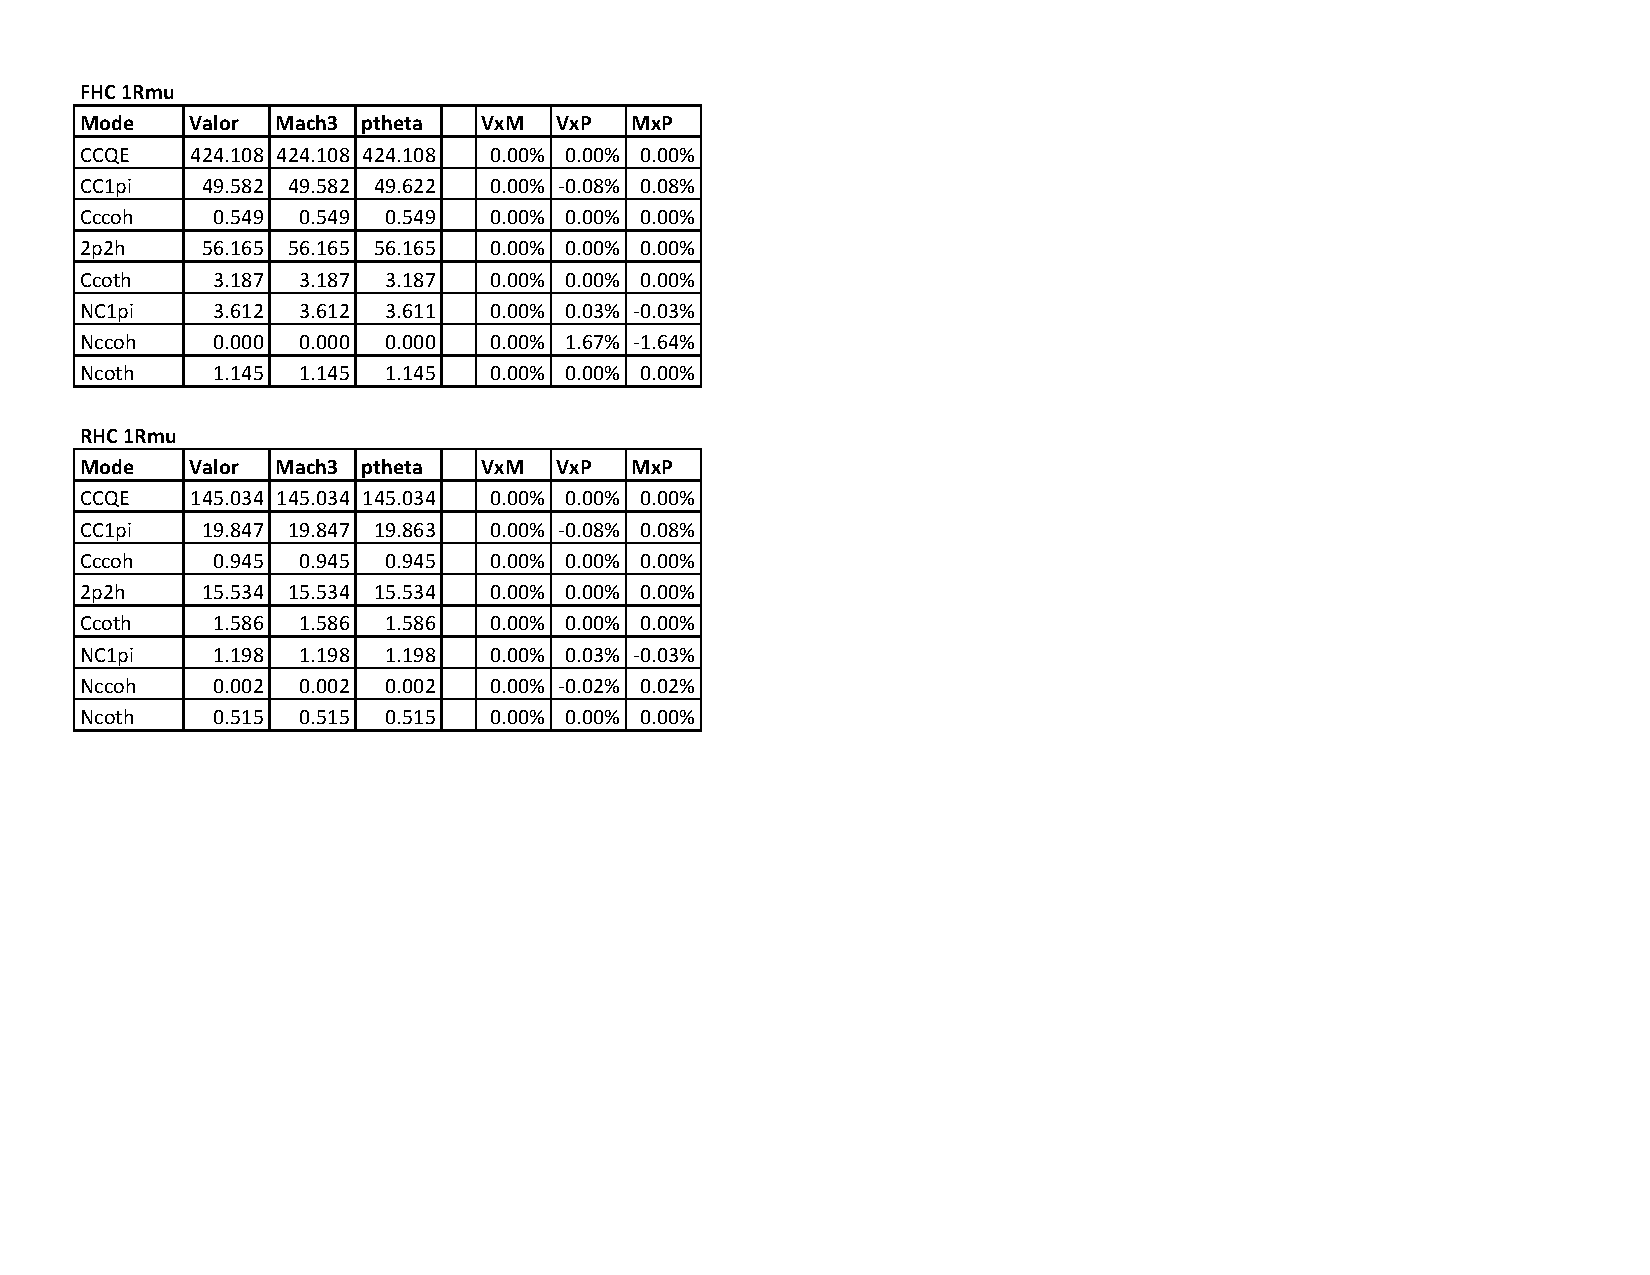
\includegraphics[page=1, trim={0cm 9cm 13cm 1cm}, clip, scale=0.52] {images/rates/prefit_unosc}
	\end{figure}
\end{frame}

\begin{frame}{Event rates: $e$-like samples pre-BANFF unoscillated}
	\centering
	\begin{figure}
		\includegraphics[page=2, trim={0cm 8cm 13cm 1cm}, clip, scale=0.52] {images/rates/prefit_unosc}
	\end{figure}
\end{frame}

\begin{frame}{Event rates: $\nu_e\text{ CC}1\pi$-like samples pre-BANFF unoscillated}
	\centering
	\begin{figure}
		\includegraphics[page=3, trim={0cm 15cm 13cm 1cm}, clip, scale=0.52] {images/rates/prefit_unosc}
	\end{figure}
\end{frame}

%===============================================================================
\section{Event rates pre-BANFF oscillated}
\begin{frame}
	\centering
	\Large Pre-BANFF oscillated event rate validation\\(Run 1-7c POT)
\end{frame}

\begin{frame}{Event rates: $\mu$-like samples pre-BANFF oscillated}
	\centering

	\begin{columns}
		\begin{column}{0.5\paperwidth}
			\begin{figure}
				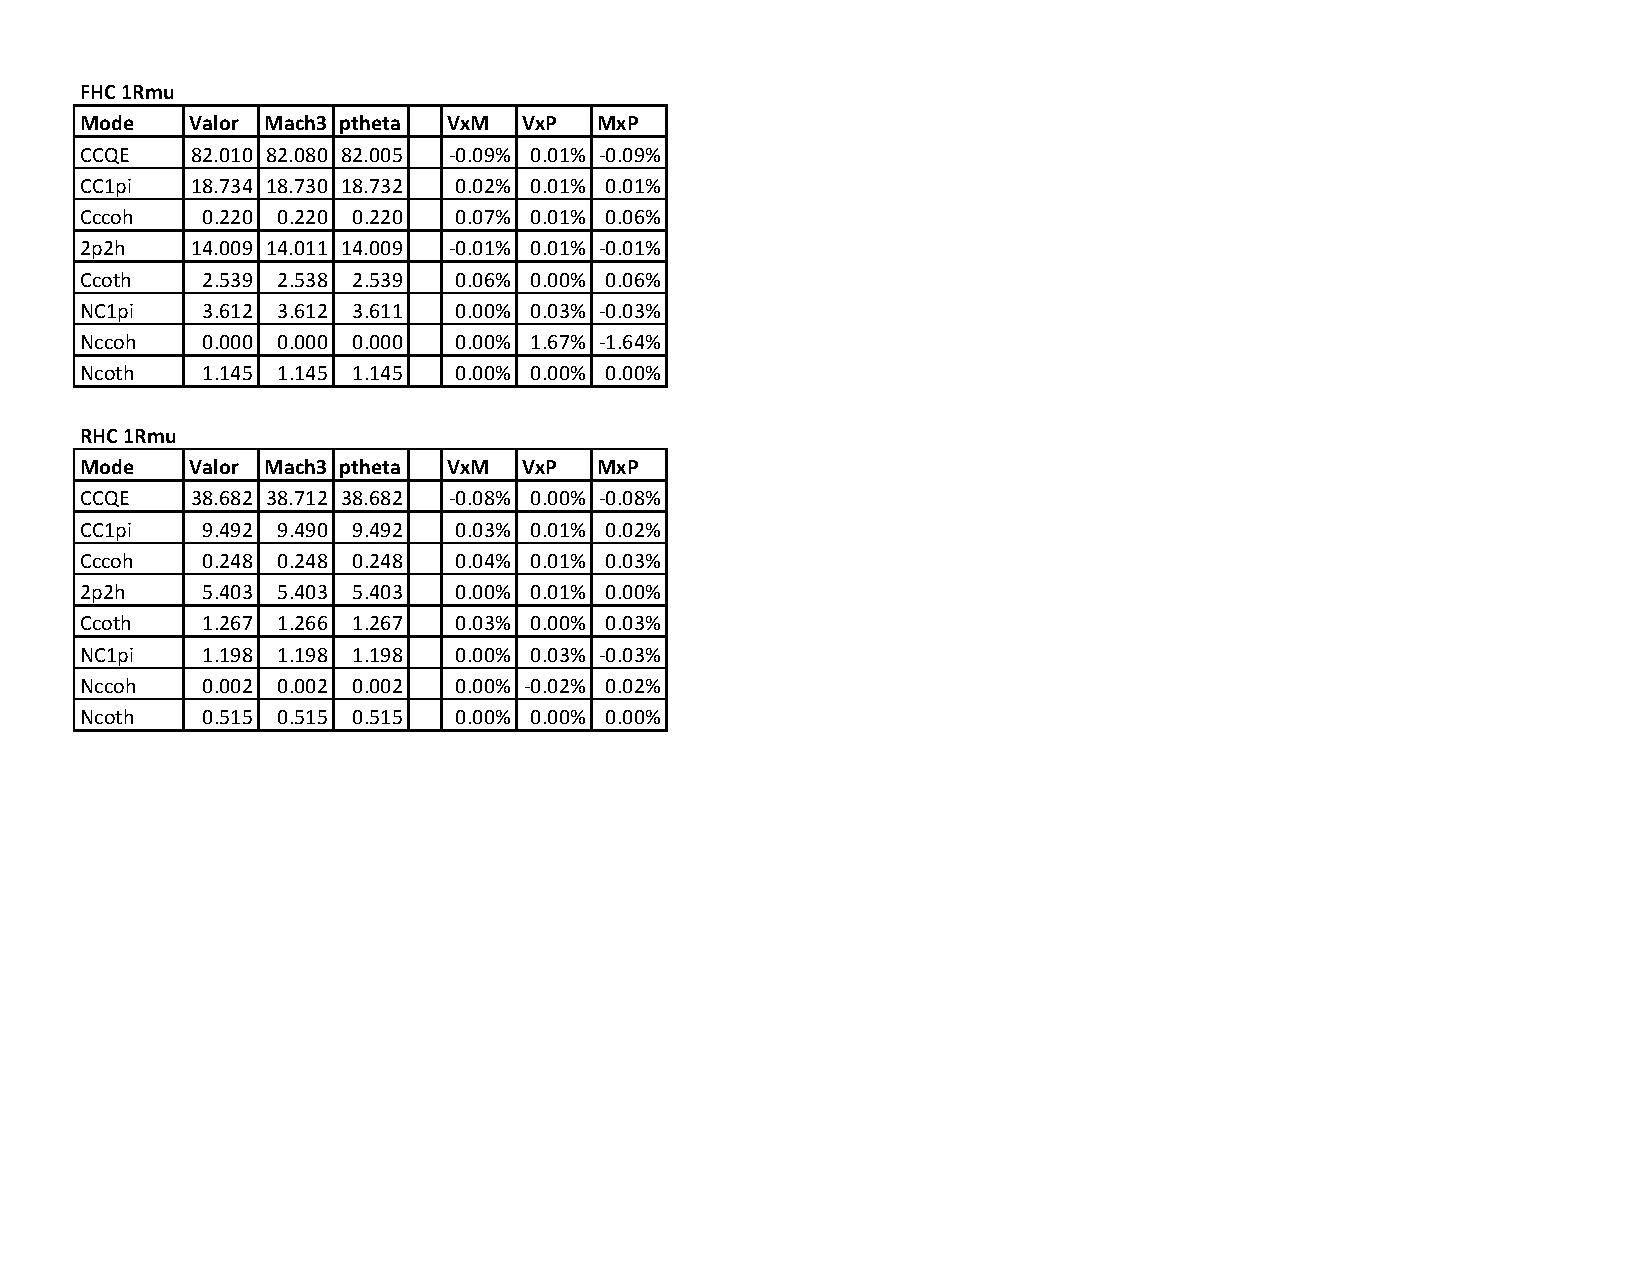
\includegraphics[page=1, trim={0cm 9cm 13cm 1cm}, clip, scale=0.52] {images/rates/prefit_A}
				\caption*{Asimov A}
			\end{figure}
		\end{column}
		\begin{column}{0.5\paperwidth}
			\begin{figure}
				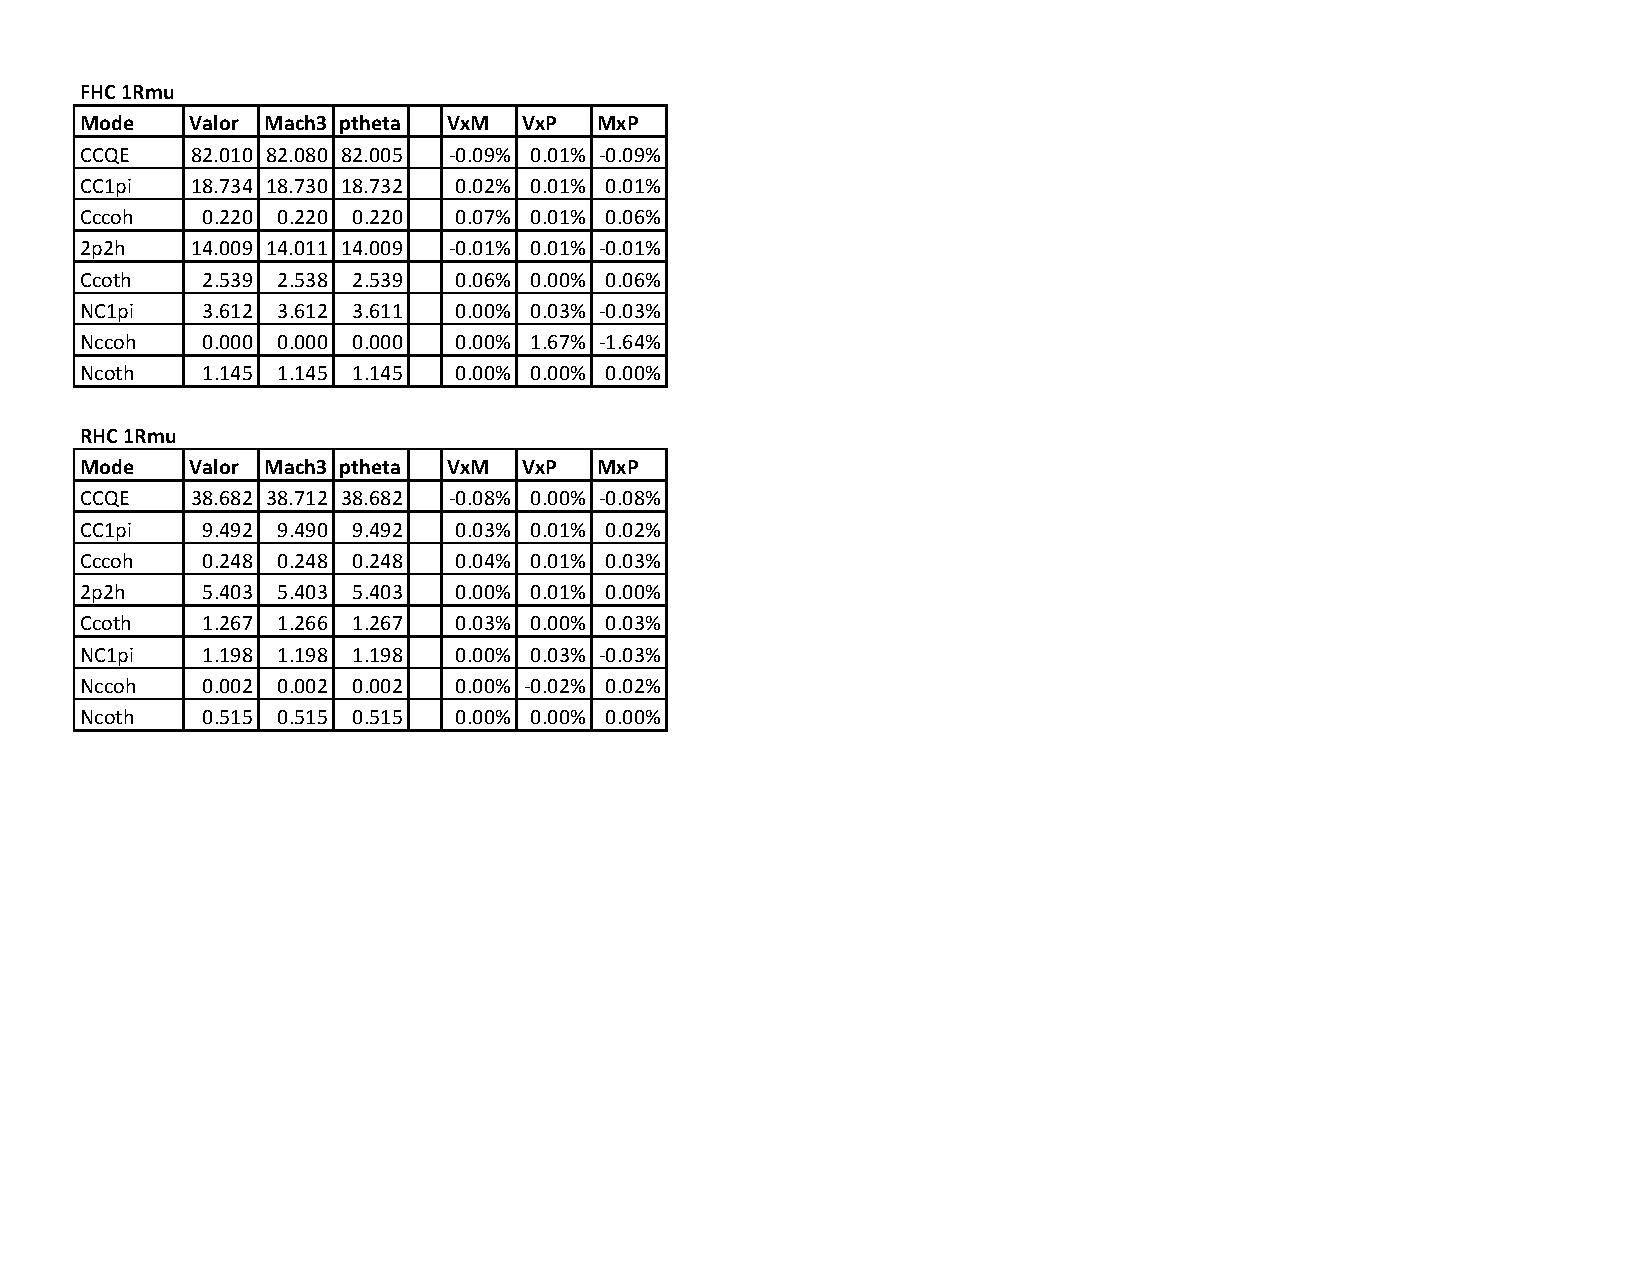
\includegraphics[page=1, trim={0cm 9cm 13cm 1cm}, clip, scale=0.52] {images/rates/prefit_A}
				\caption*{Asimov B}
			\end{figure}
		\end{column}
	\end{columns}
\end{frame}

\begin{frame}{Event rates: $e$-like samples pre-BANFF oscillated}
	\centering

	\begin{columns}
		\begin{column}{0.5\paperwidth}
			\begin{figure}
				\includegraphics[page=2, trim={0cm 8cm 13cm 1cm}, clip, scale=0.52] {images/rates/prefit_A}
				\caption*{Asimov A}
			\end{figure}
		\end{column}
		\begin{column}{0.5\paperwidth}
			\begin{figure}
				\includegraphics[page=2, trim={0cm 8cm 13cm 1cm}, clip, scale=0.52] {images/rates/prefit_A}
				\caption*{Asimov B}
			\end{figure}
		\end{column}
	\end{columns}
\end{frame}

\begin{frame}{Event rates: $\nu_e\text{ CC}1\pi$-like samples pre-BANFF oscillated}
	\centering

	\begin{columns}
		\begin{column}{0.5\paperwidth}
			\begin{figure}
				\includegraphics[page=3, trim={0cm 15cm 13cm 1cm}, clip, scale=0.52] {images/rates/prefit_A}
				\caption*{Asimov A}
			\end{figure}
		\end{column}
		\begin{column}{0.5\paperwidth}
			\begin{figure}
				\includegraphics[page=3, trim={0cm 15cm 13cm 1cm}, clip, scale=0.52] {images/rates/prefit_A}
				\caption*{Asimov B}
			\end{figure}
		\end{column}
	\end{columns}
\end{frame}

%===============================================================================
\section{Event rates post-BANFF unoscillated}
\begin{frame}
	\centering
	\Large Post-BANFF unoscillated event rate validation\\(Run 1-7c POT)
\end{frame}

\begin{frame}{Event rates: $\mu$-like samples post-BANFF unoscillated}
	\centering
	\begin{figure}
		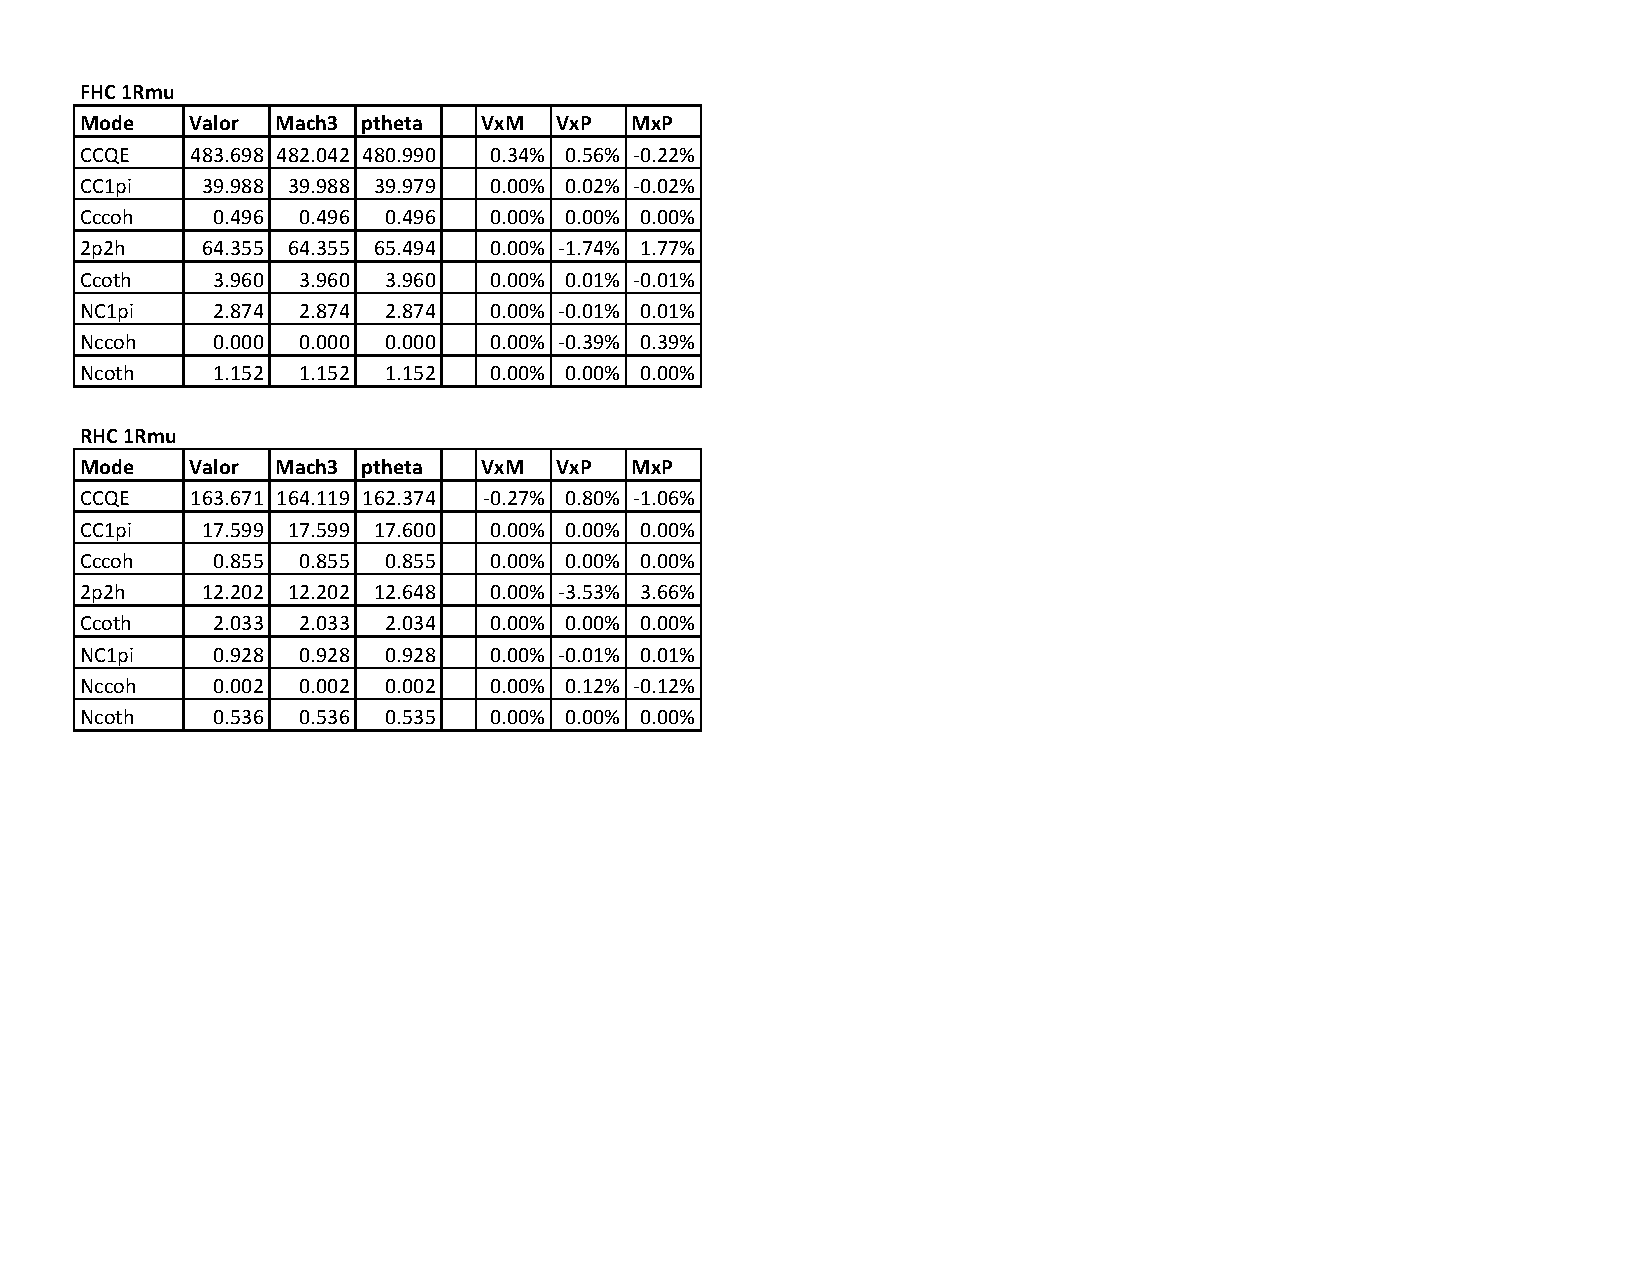
\includegraphics[page=1, trim={0cm 9cm 13cm 1cm}, clip, scale=0.52] {images/rates/postfit_unosc}
	\end{figure}
\end{frame}

\begin{frame}{Event rates: $e$-like samples post-BANFF unoscillated}
	\centering
	\begin{figure}
		\includegraphics[page=2, trim={0cm 8cm 13cm 1cm}, clip, scale=0.52] {images/rates/postfit_unosc}
	\end{figure}
\end{frame}

\begin{frame}{Event rates: $\nu_e\text{ CC}1\pi$-like samples post-BANFF unoscillated}
	\centering
	\begin{figure}
		\includegraphics[page=3, trim={0cm 15cm 13cm 1cm}, clip, scale=0.52] {images/rates/postfit_unosc}
	\end{figure}
\end{frame}

%===============================================================================
\section{Event rates post-BANFF oscillated}
\begin{frame}
	\centering
	\Large Post-BANFF oscillated event rate validation\\(Run 1-7c POT)
\end{frame}

\begin{frame}{Event rates: $\mu$-like samples post-BANFF oscillated}
	\centering

	\begin{columns}
		\begin{column}{0.5\paperwidth}
			\begin{figure}
				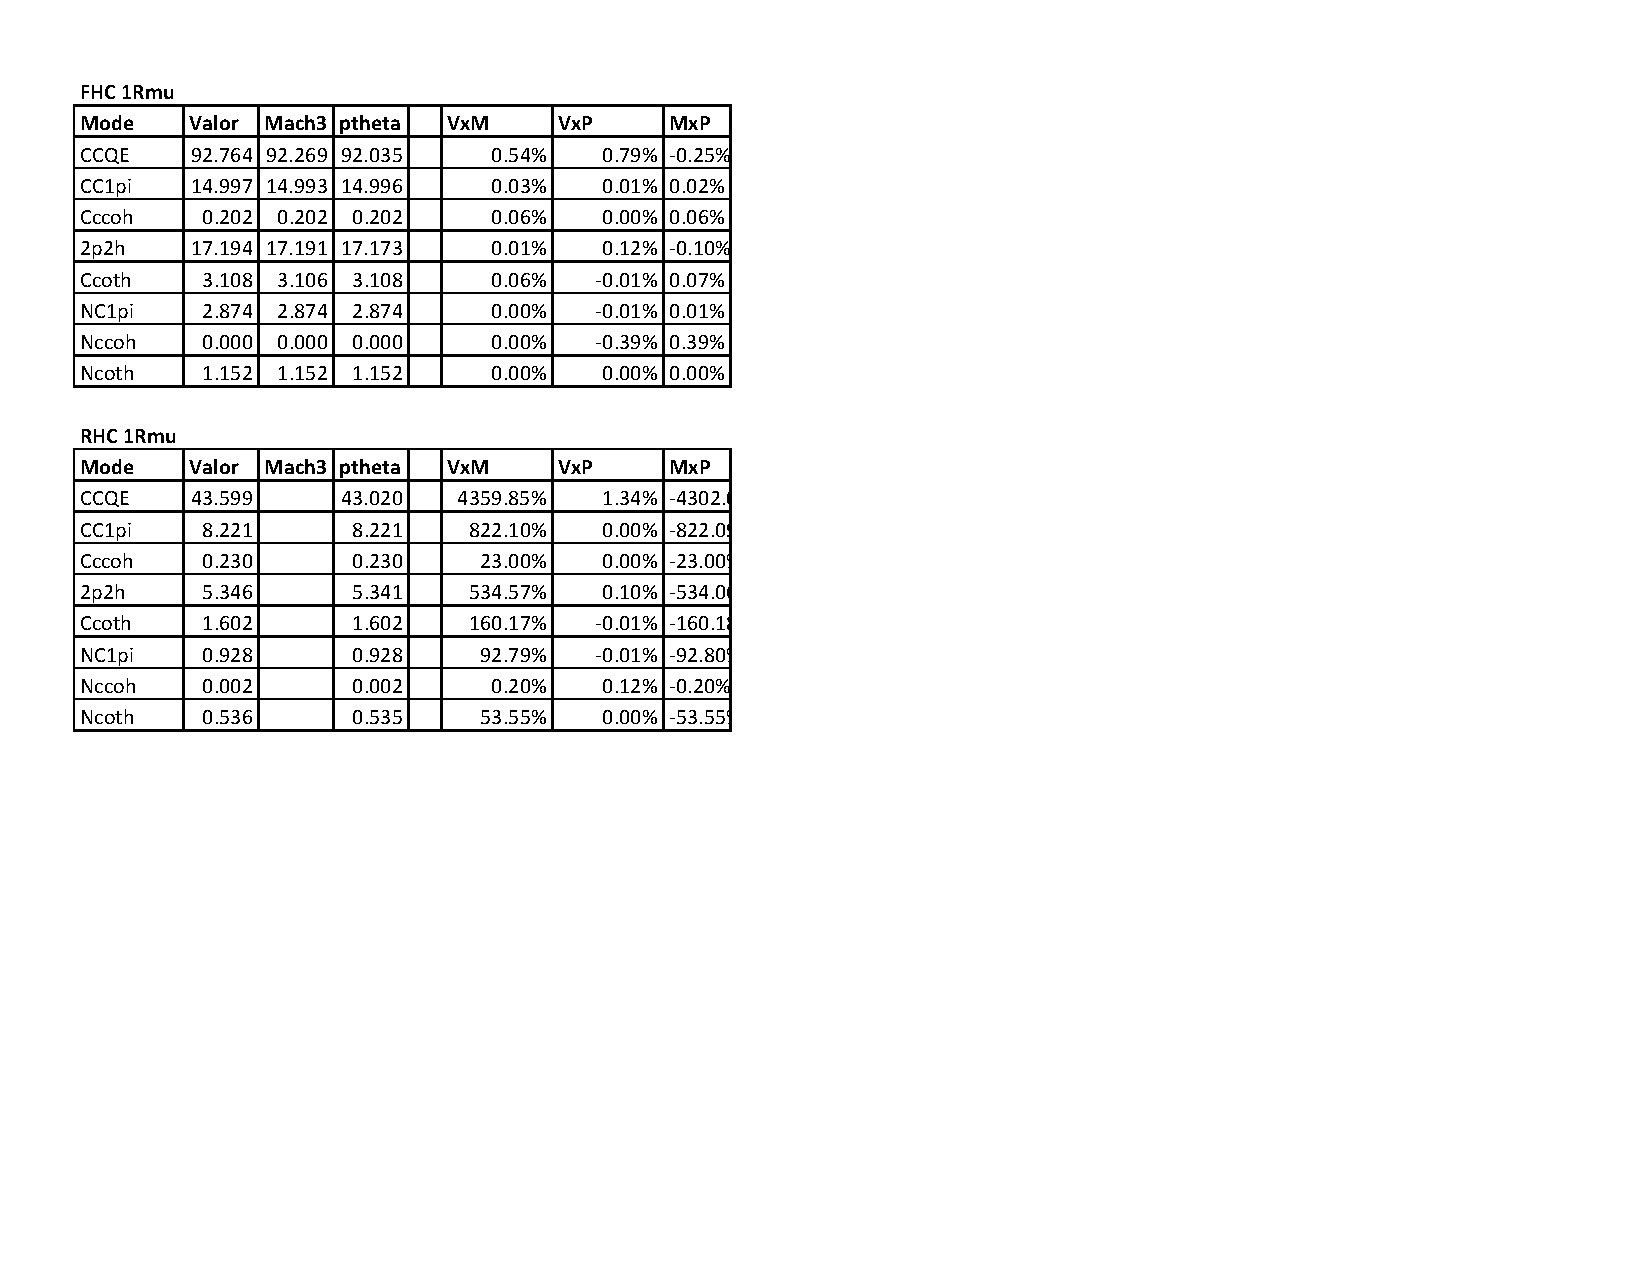
\includegraphics[page=1, trim={0cm 9cm 13cm 1cm}, clip, scale=0.52] {images/rates/postfit_A}
				\caption*{Asimov A}
			\end{figure}
		\end{column}
		\begin{column}{0.5\paperwidth}
			\begin{figure}
				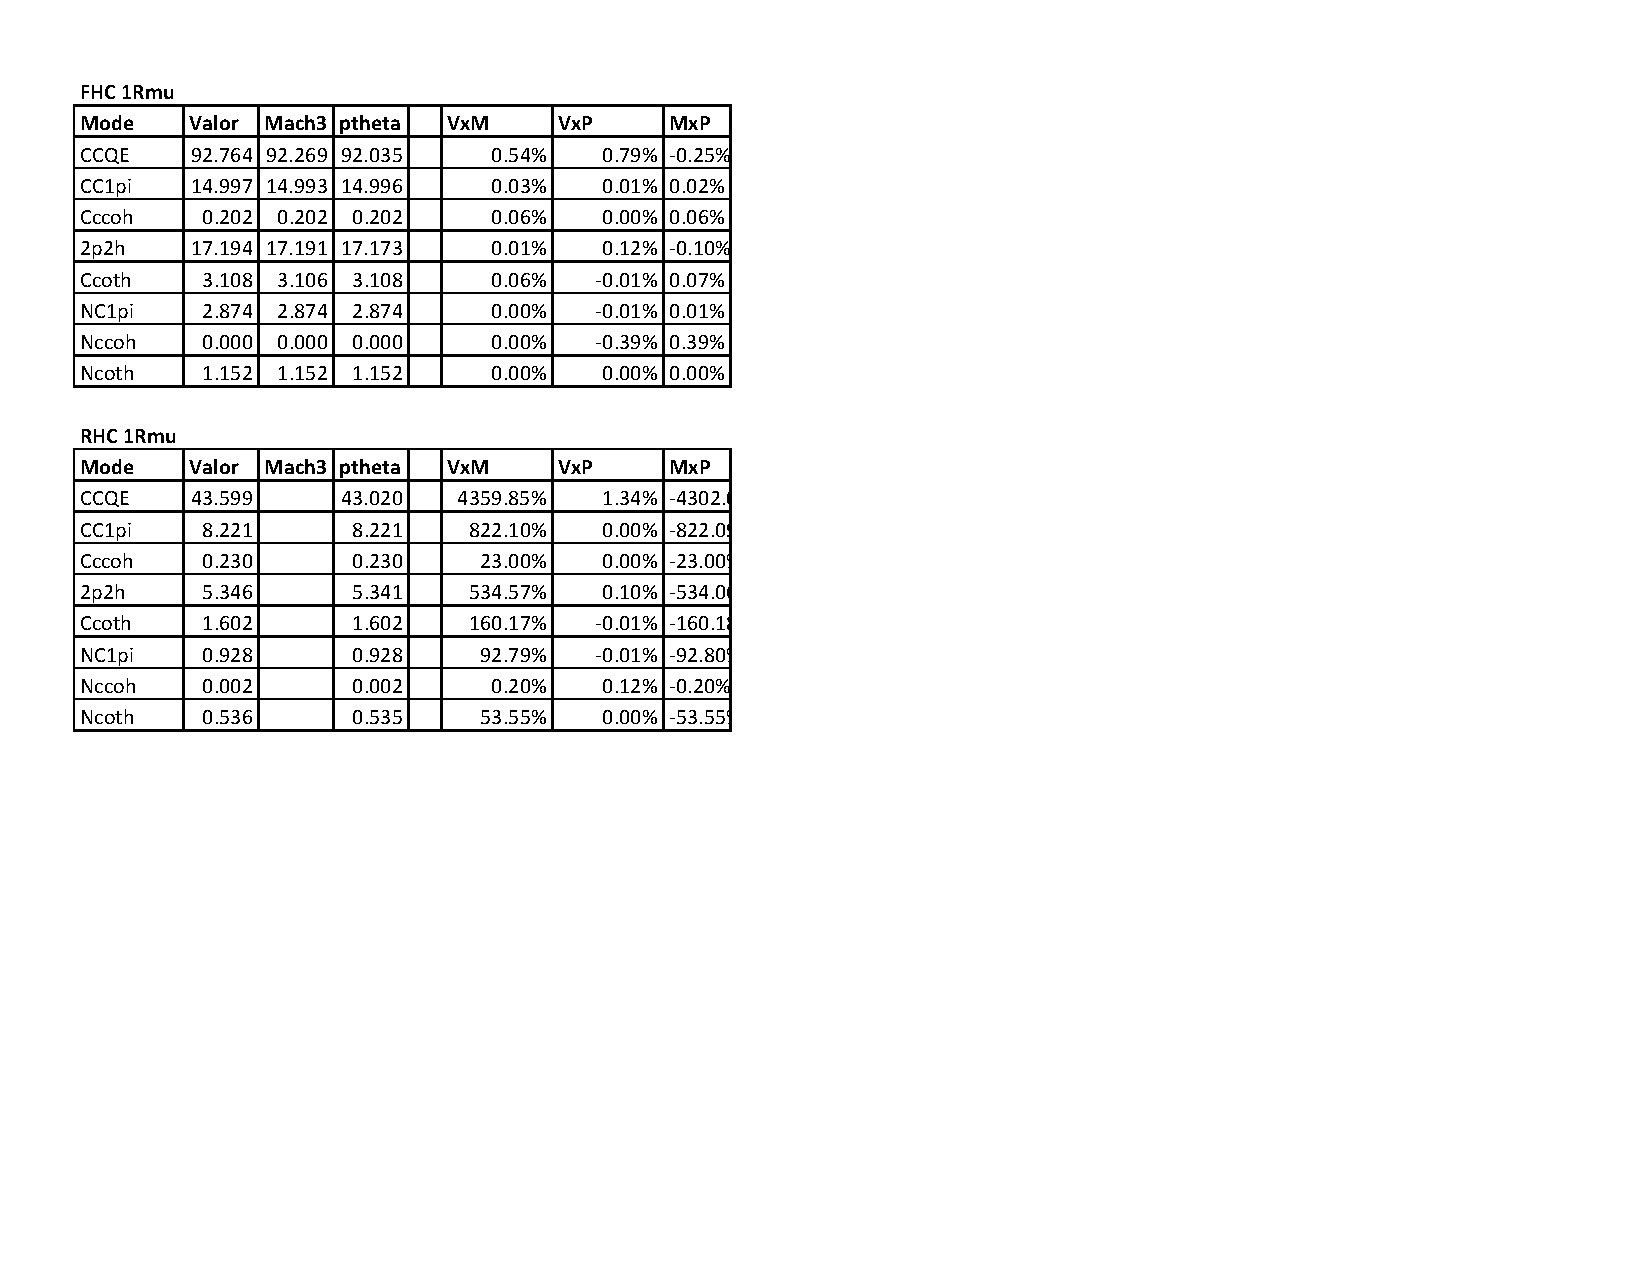
\includegraphics[page=1, trim={0cm 9cm 13cm 1cm}, clip, scale=0.52] {images/rates/postfit_A}
				\caption*{Asimov B}
			\end{figure}
		\end{column}
	\end{columns}
\end{frame}

\begin{frame}{Event rates: $e$-like samples post-BANFF oscillated}
	\centering

	\begin{columns}
		\begin{column}{0.5\paperwidth}
			\begin{figure}
				\includegraphics[page=2, trim={0cm 8cm 13cm 1cm}, clip, scale=0.52] {images/rates/postfit_A}
				\caption*{Asimov A}
			\end{figure}
		\end{column}
		\begin{column}{0.5\paperwidth}
			\begin{figure}
				\includegraphics[page=2, trim={0cm 8cm 13cm 1cm}, clip, scale=0.52] {images/rates/postfit_A}
				\caption*{Asimov B}
			\end{figure}
		\end{column}
	\end{columns}
\end{frame}

\begin{frame}{Event rates: $\nu_e\text{ CC}1\pi$-like samples post-BANFF oscillated}
	\centering
	\begin{columns}
		\begin{column}{0.5\paperwidth}
			\begin{figure}
				\includegraphics[page=3, trim={0cm 15cm 13cm 1cm}, clip, scale=0.52] {images/rates/postfit_A}
				\caption*{Asimov A}
			\end{figure}
		\end{column}
		\begin{column}{0.5\paperwidth}
			\begin{figure}
				\includegraphics[page=3, trim={0cm 15cm 13cm 1cm}, clip, scale=0.52] {images/rates/postfit_A}
				\caption*{Asimov B}
			\end{figure}
		\end{column}
	\end{columns}
\end{frame}

%===============================================================================
\section{Systematic variations validation}
\begin{frame}
	\centering
	\Large Pre-BANFF systematic variations validation\\(Run 1-7c POT)
\end{frame}

\begin{frame}{Example spline variations: CA5}
	\centering
	\begin{columns}
		\begin{column}{0.5\paperwidth}
			\begin{figure}
				\includegraphics[page=11, trim={0cm 0cm 0cm 0cm}, clip, scale=0.35] {images/variations/valor_mach3/variations_prebanff_unosc_1Re}
				\caption*{VALOR vs MaCh3}
			\end{figure}
		\end{column}
		\begin{column}{0.5\paperwidth}
			\begin{figure}
				\includegraphics[page=7, trim={0cm 0cm 0cm 0cm}, clip, scale=0.35] {images/variations/valor_ptheta/variations_prebanff_unosc_1Re}
				\caption*{VALOR vs p-theta}
			\end{figure}
		\end{column}
	\end{columns}
\end{frame}

\begin{frame}{Example normalisation variations: $\mu$-like CC coherent}
	\centering
	\begin{columns}
		\begin{column}{0.5\paperwidth}
			\begin{figure}
				\includegraphics[page=17, trim={0cm 0cm 0cm 0cm}, clip, scale=0.35] {images/variations/valor_mach3/variations_prebanff_unosc_1Re}
				\caption*{VALOR vs MaCh3}
			\end{figure}
		\end{column}
		\begin{column}{0.5\paperwidth}
			\begin{figure}
				\includegraphics[page=13, trim={0cm 0cm 0cm 0cm}, clip, scale=0.35] {images/variations/valor_ptheta/variations_prebanff_unosc_1Re}
				\caption*{VALOR vs p-theta}
			\end{figure}
		\end{column}
	\end{columns}
\end{frame}

\begin{frame}{BeRPA variations: BeRPA A}
	\centering
	\begin{columns}
		\begin{column}{0.5\paperwidth}
			\begin{figure}
				\includegraphics[page=7, trim={0cm 0cm 0cm 0cm}, clip, scale=0.35] {images/variations/valor_mach3/variations_prebanff_unosc_1Re}
				\caption*{VALOR vs MaCh3}
			\end{figure}
		\end{column}
		\begin{column}{0.5\paperwidth}
			\begin{figure}
				\includegraphics[page=17, trim={0cm 0cm 0cm 0cm}, clip, scale=0.35] {images/variations/valor_ptheta/variations_prebanff_unosc_1Re}
				\caption*{VALOR vs p-theta}
			\end{figure}
		\end{column}
	\end{columns}
\end{frame}

\begin{frame}{BeRPA variations: BeRPA B}
	\centering
	\begin{columns}
		\begin{column}{0.5\paperwidth}
			\begin{figure}
				\includegraphics[page=8, trim={0cm 0cm 0cm 0cm}, clip, scale=0.35] {images/variations/valor_mach3/variations_prebanff_unosc_1Re}
				\caption*{VALOR vs MaCh3}
			\end{figure}
		\end{column}
		\begin{column}{0.5\paperwidth}
			\begin{figure}
				\includegraphics[page=18, trim={0cm 0cm 0cm 0cm}, clip, scale=0.35] {images/variations/valor_ptheta/variations_prebanff_unosc_1Re}
				\caption*{VALOR vs p-theta}
			\end{figure}
		\end{column}
	\end{columns}
\end{frame}

\begin{frame}{BeRPA variations: BeRPA D}
	\centering
	\begin{columns}
		\begin{column}{0.5\paperwidth}
			\begin{figure}
				\includegraphics[page=9, trim={0cm 0cm 0cm 0cm}, clip, scale=0.35] {images/variations/valor_mach3/variations_prebanff_unosc_1Re}
				\caption*{VALOR vs MaCh3}
			\end{figure}
		\end{column}
		\begin{column}{0.5\paperwidth}
			\begin{figure}
				\includegraphics[page=19, trim={0cm 0cm 0cm 0cm}, clip, scale=0.35] {images/variations/valor_ptheta/variations_prebanff_unosc_1Re}
				\caption*{VALOR vs p-theta}
			\end{figure}
		\end{column}
	\end{columns}
\end{frame}

\begin{frame}{BeRPA variations: BeRPA E}
	\centering
	\begin{columns}
		\begin{column}{0.5\paperwidth}
			\begin{figure}
				\includegraphics[page=10, trim={0cm 0cm 0cm 0cm}, clip, scale=0.35] {images/variations/valor_mach3/variations_prebanff_unosc_1Re}
				\caption*{VALOR vs MaCh3}
			\end{figure}
		\end{column}
		\begin{column}{0.5\paperwidth}
			\begin{figure}
				\includegraphics[page=20, trim={0cm 0cm 0cm 0cm}, clip, scale=0.35] {images/variations/valor_ptheta/variations_prebanff_unosc_1Re}
				\caption*{VALOR vs p-theta}
			\end{figure}
		\end{column}
	\end{columns}
\end{frame}

%===============================================================================
\section{Conclusion}
\begin{frame}{Conclusion}
	\centering
	\begin{itemize}
		\item Good agreement between VALOR and MaCh3 in rates and variations
		\item p-theta differences under investigation
	\end{itemize}
\end{frame}

%===============================================================================
\section{Backup}
\begin{frame}
	\centering
	\Large Backup
\end{frame}

%===============================================================================
\section{Error tables}
\begin{frame}
	\centering
	\Large Systematic variations tables
\end{frame}

\begin{frame}{FHC $\mu$-like pre-BANFF unoscillated}
	\centering
	\begin{figure}
		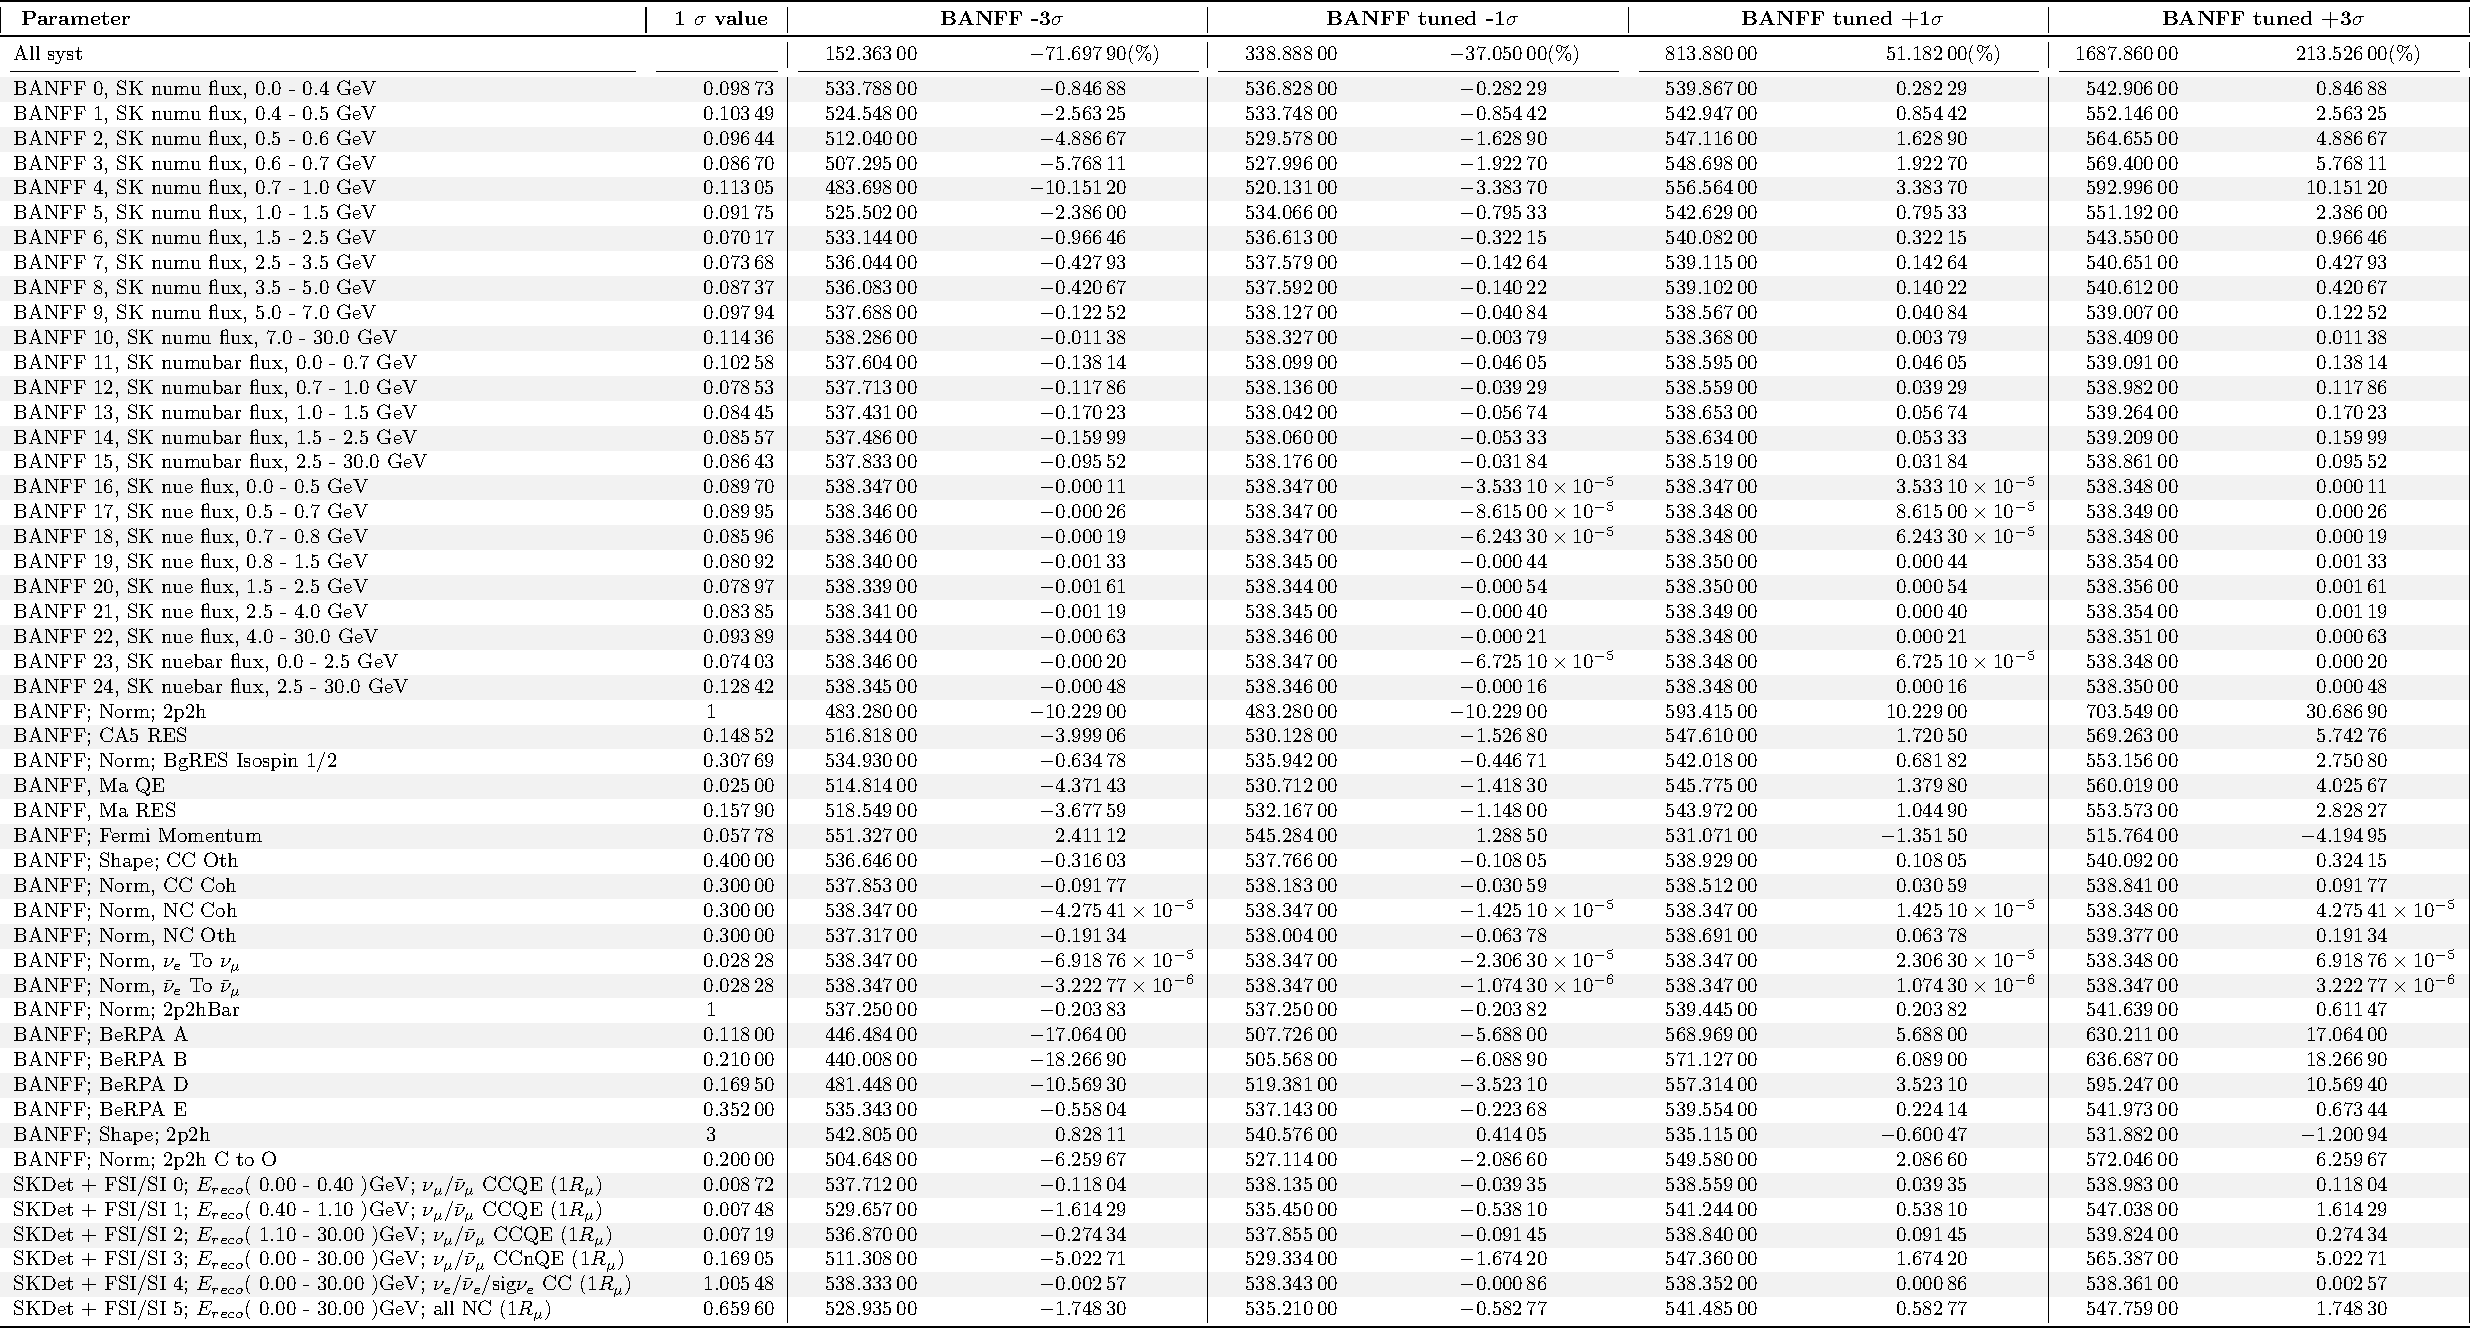
\includegraphics[page=1, trim={0cm 0cm 0cm 0cm}, clip, scale=0.25] {images/variations/tables/systematic_tables_prefit_unosc_1Rmu}
	\end{figure}
\end{frame}

\begin{frame}{FHC $e$-like pre-BANFF unoscillated}
	\centering
	\begin{figure}
		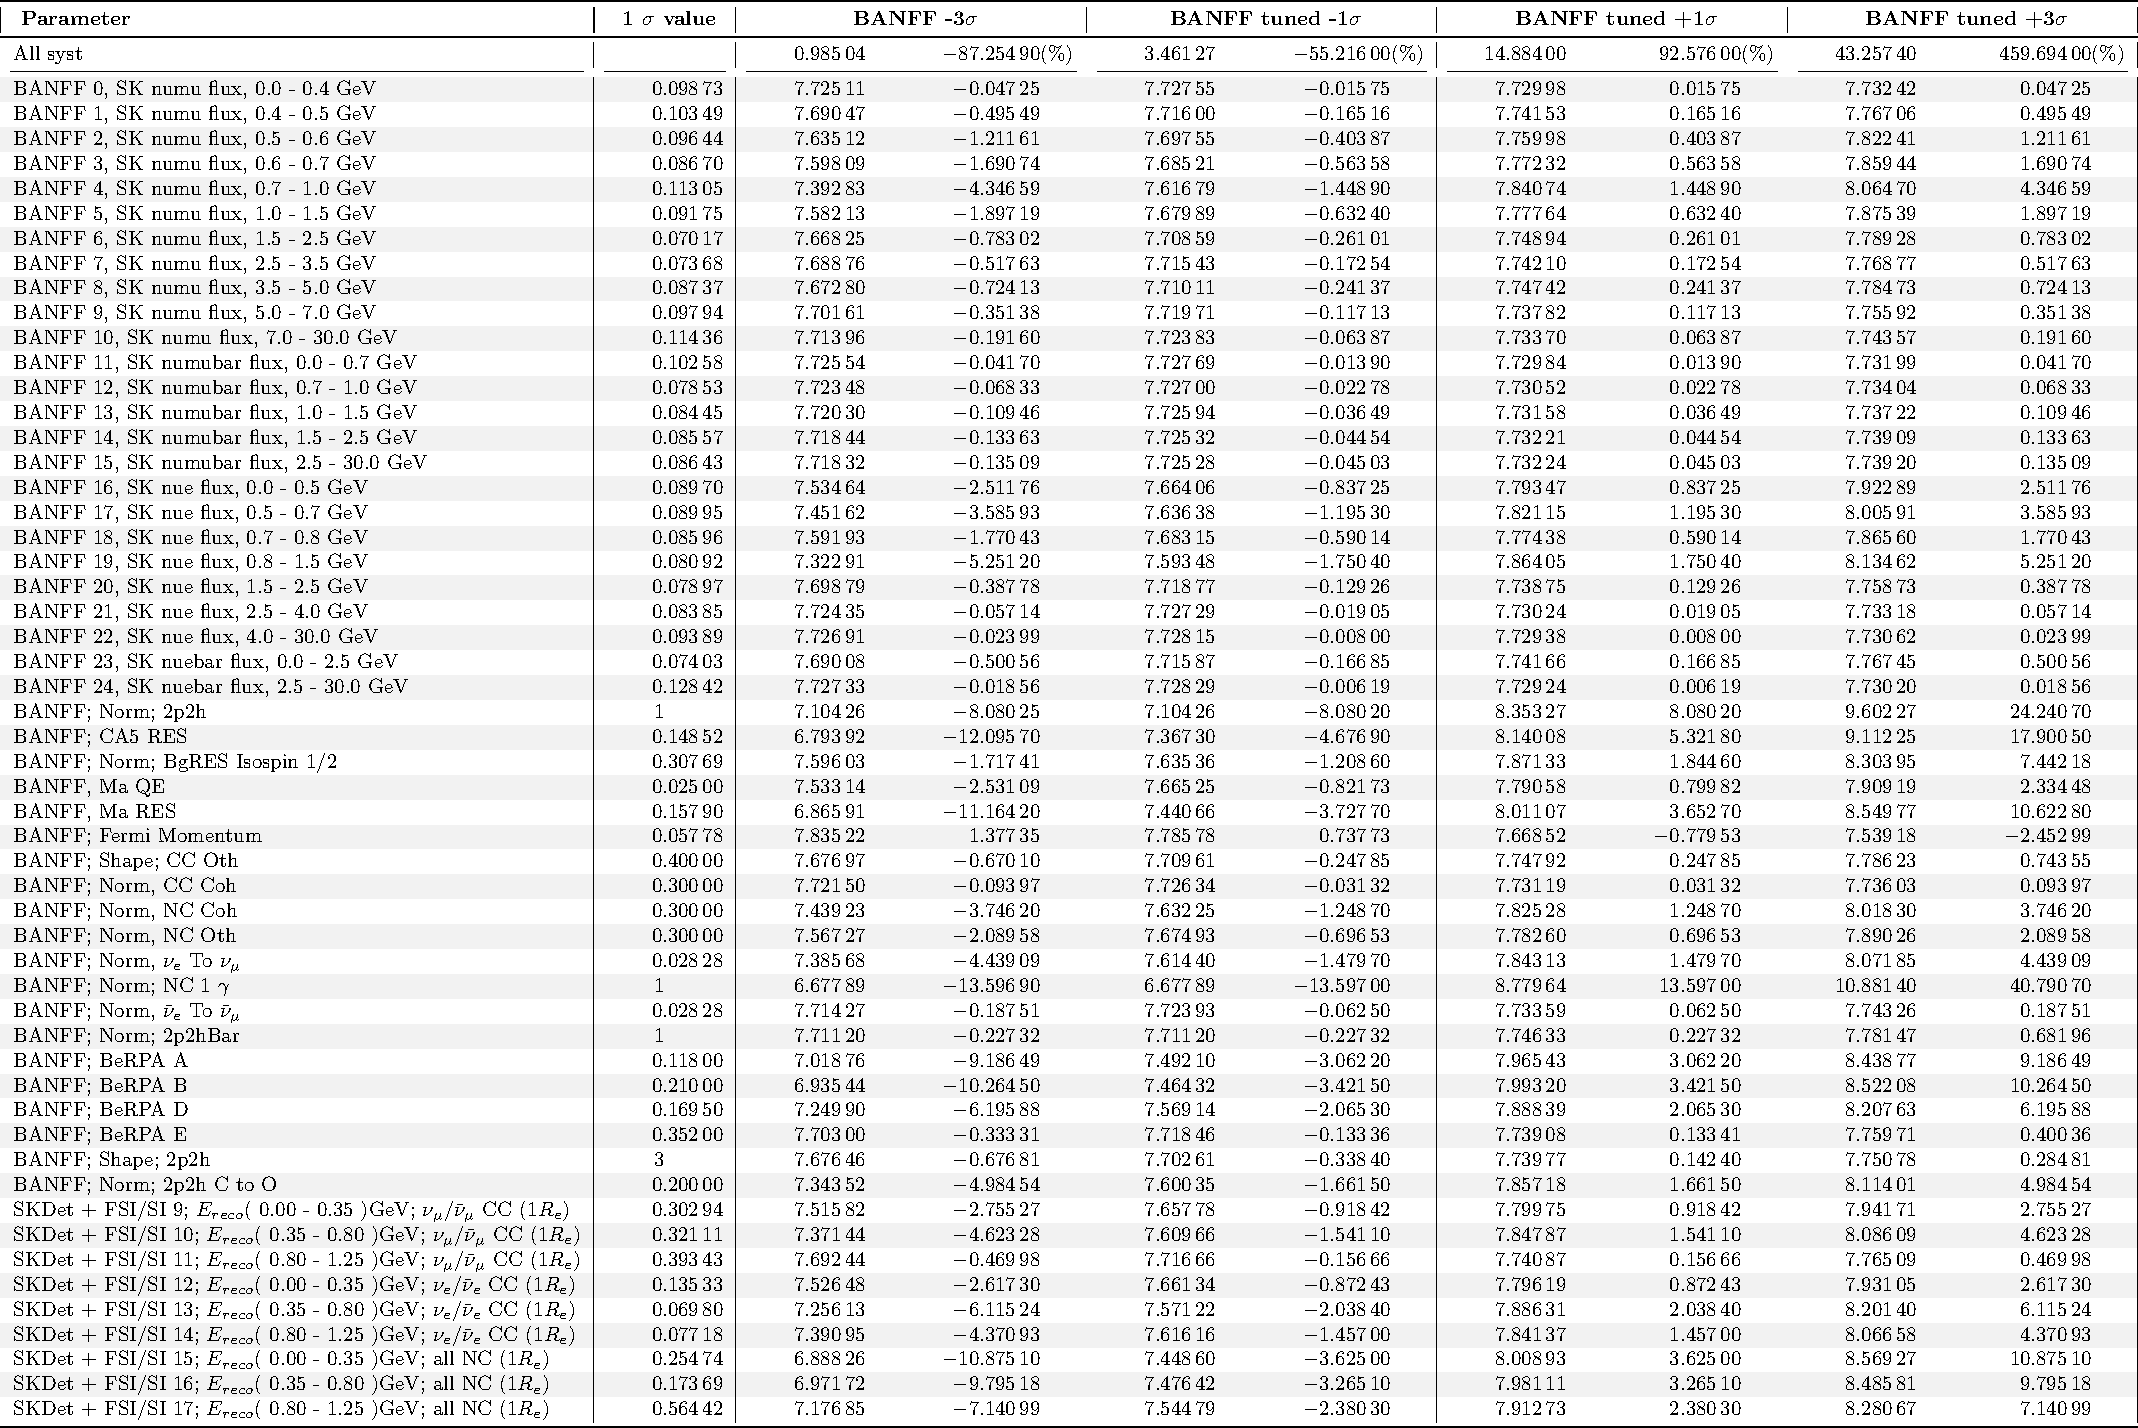
\includegraphics[page=1, trim={0cm 0cm 0cm 0cm}, clip, scale=0.3] {images/variations/tables/systematic_tables_prefit_unosc_1Re}
	\end{figure}
\end{frame}

\begin{frame}{FHC $\nu_e\text{ CC}1\pi$-like pre-BANFF unoscillated}
	\centering
	\begin{figure}
		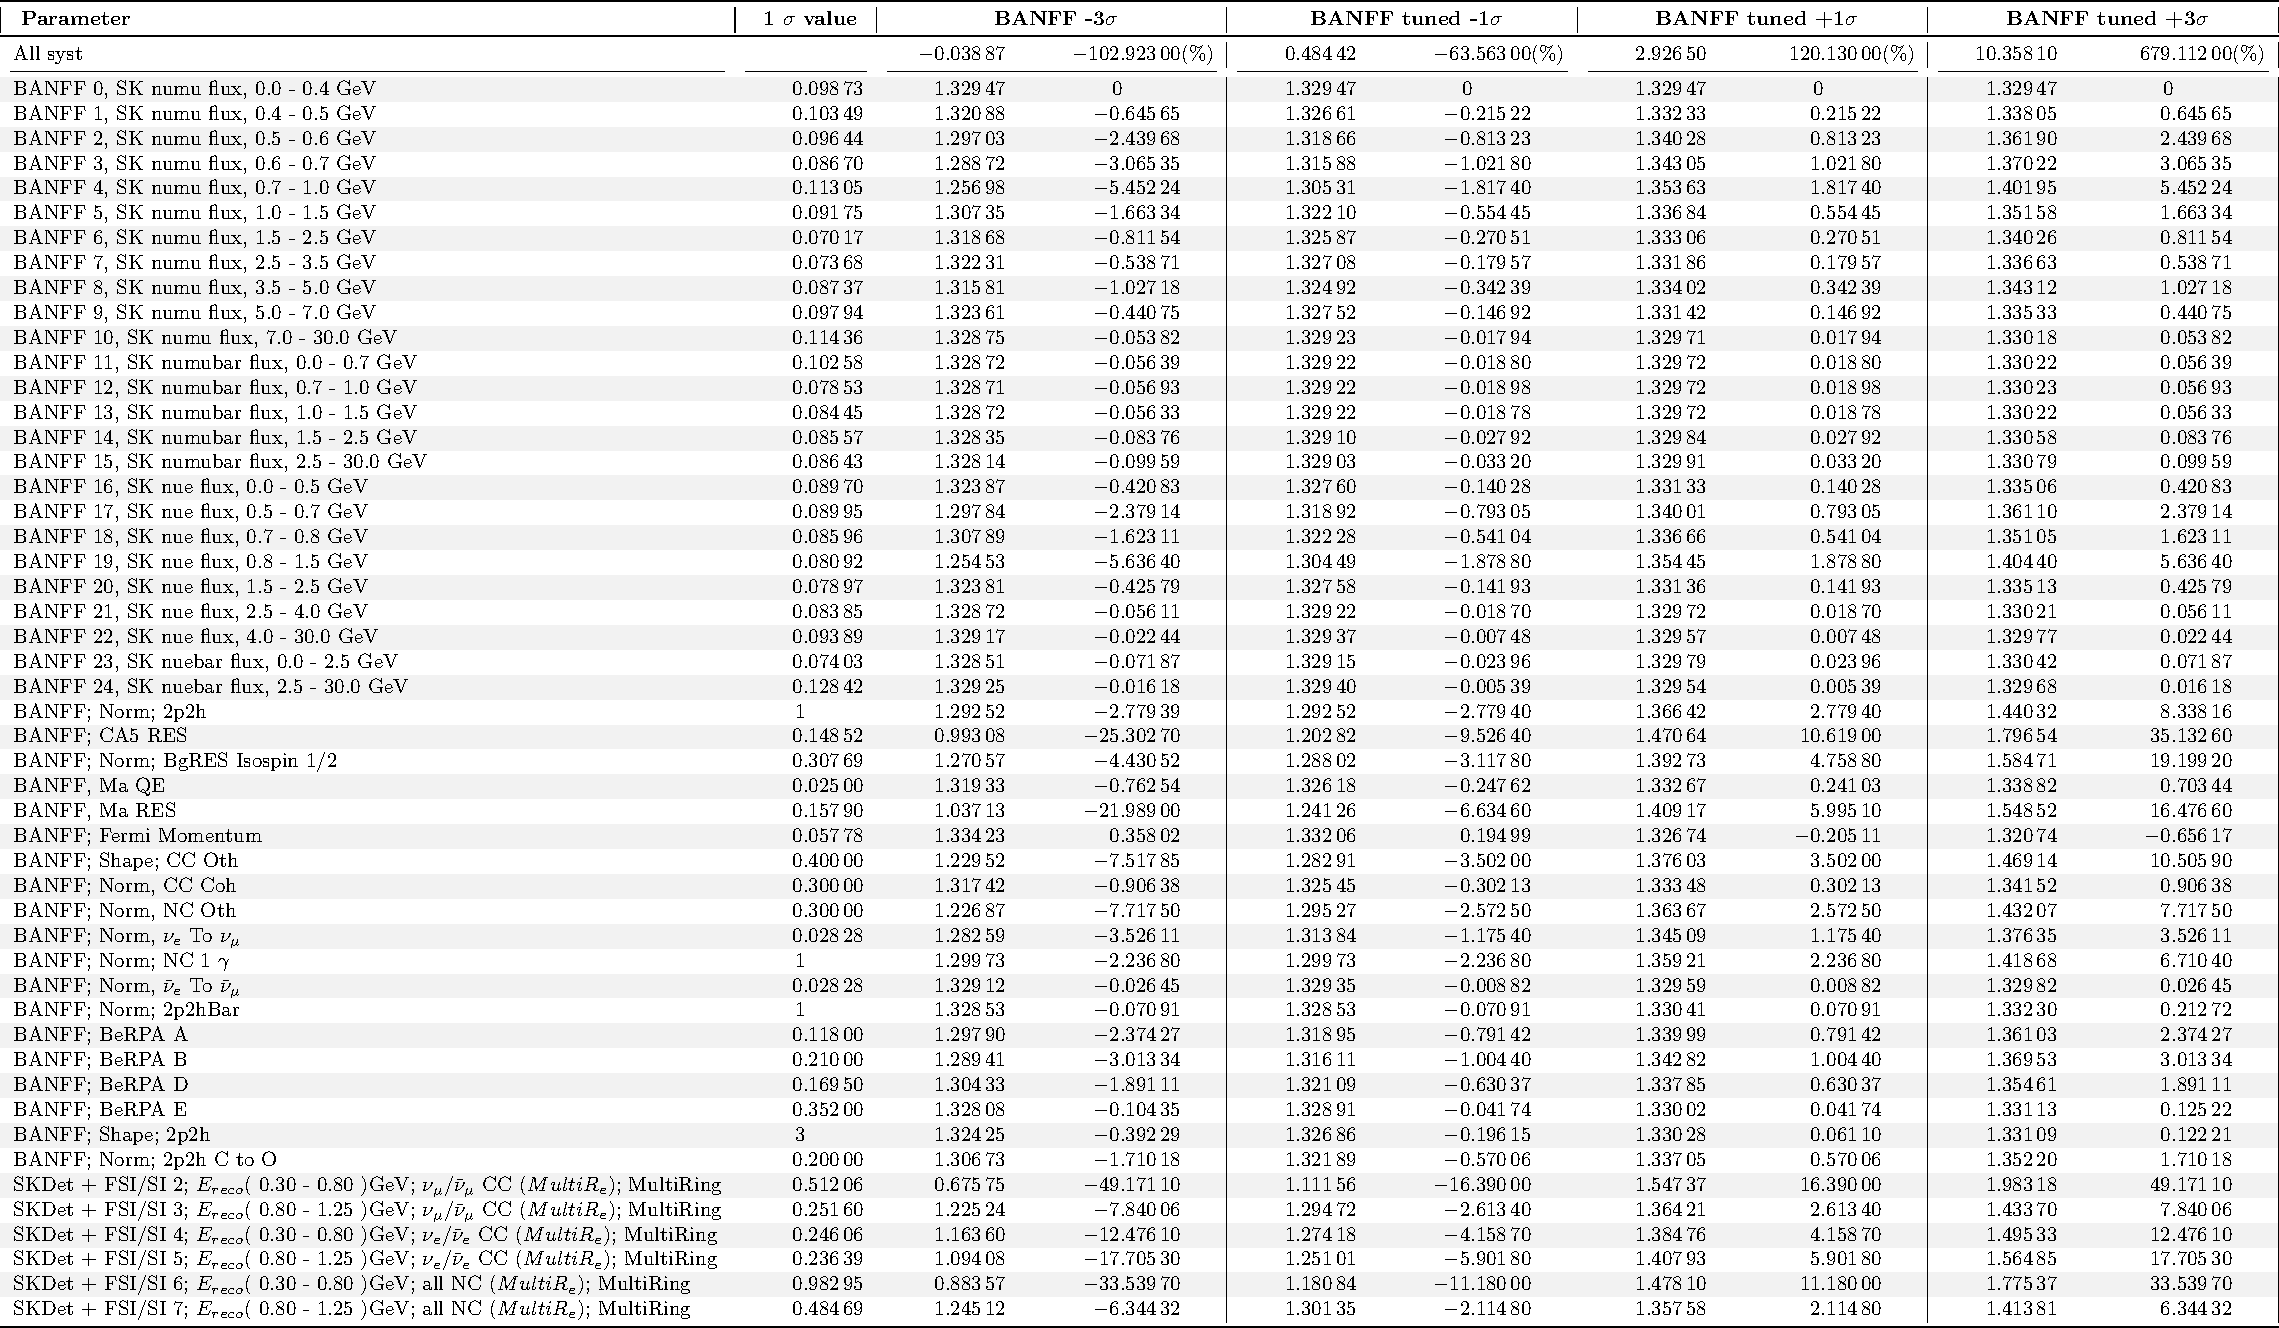
\includegraphics[page=1, trim={0cm 0cm 0cm 0cm}, clip, scale=0.28] {images/variations/tables/systematic_tables_prefit_unosc_MultiRe}
	\end{figure}
\end{frame}

\begin{frame}{RHC $\mu$-like pre-BANFF unoscillated}
	\centering
	\begin{figure}
		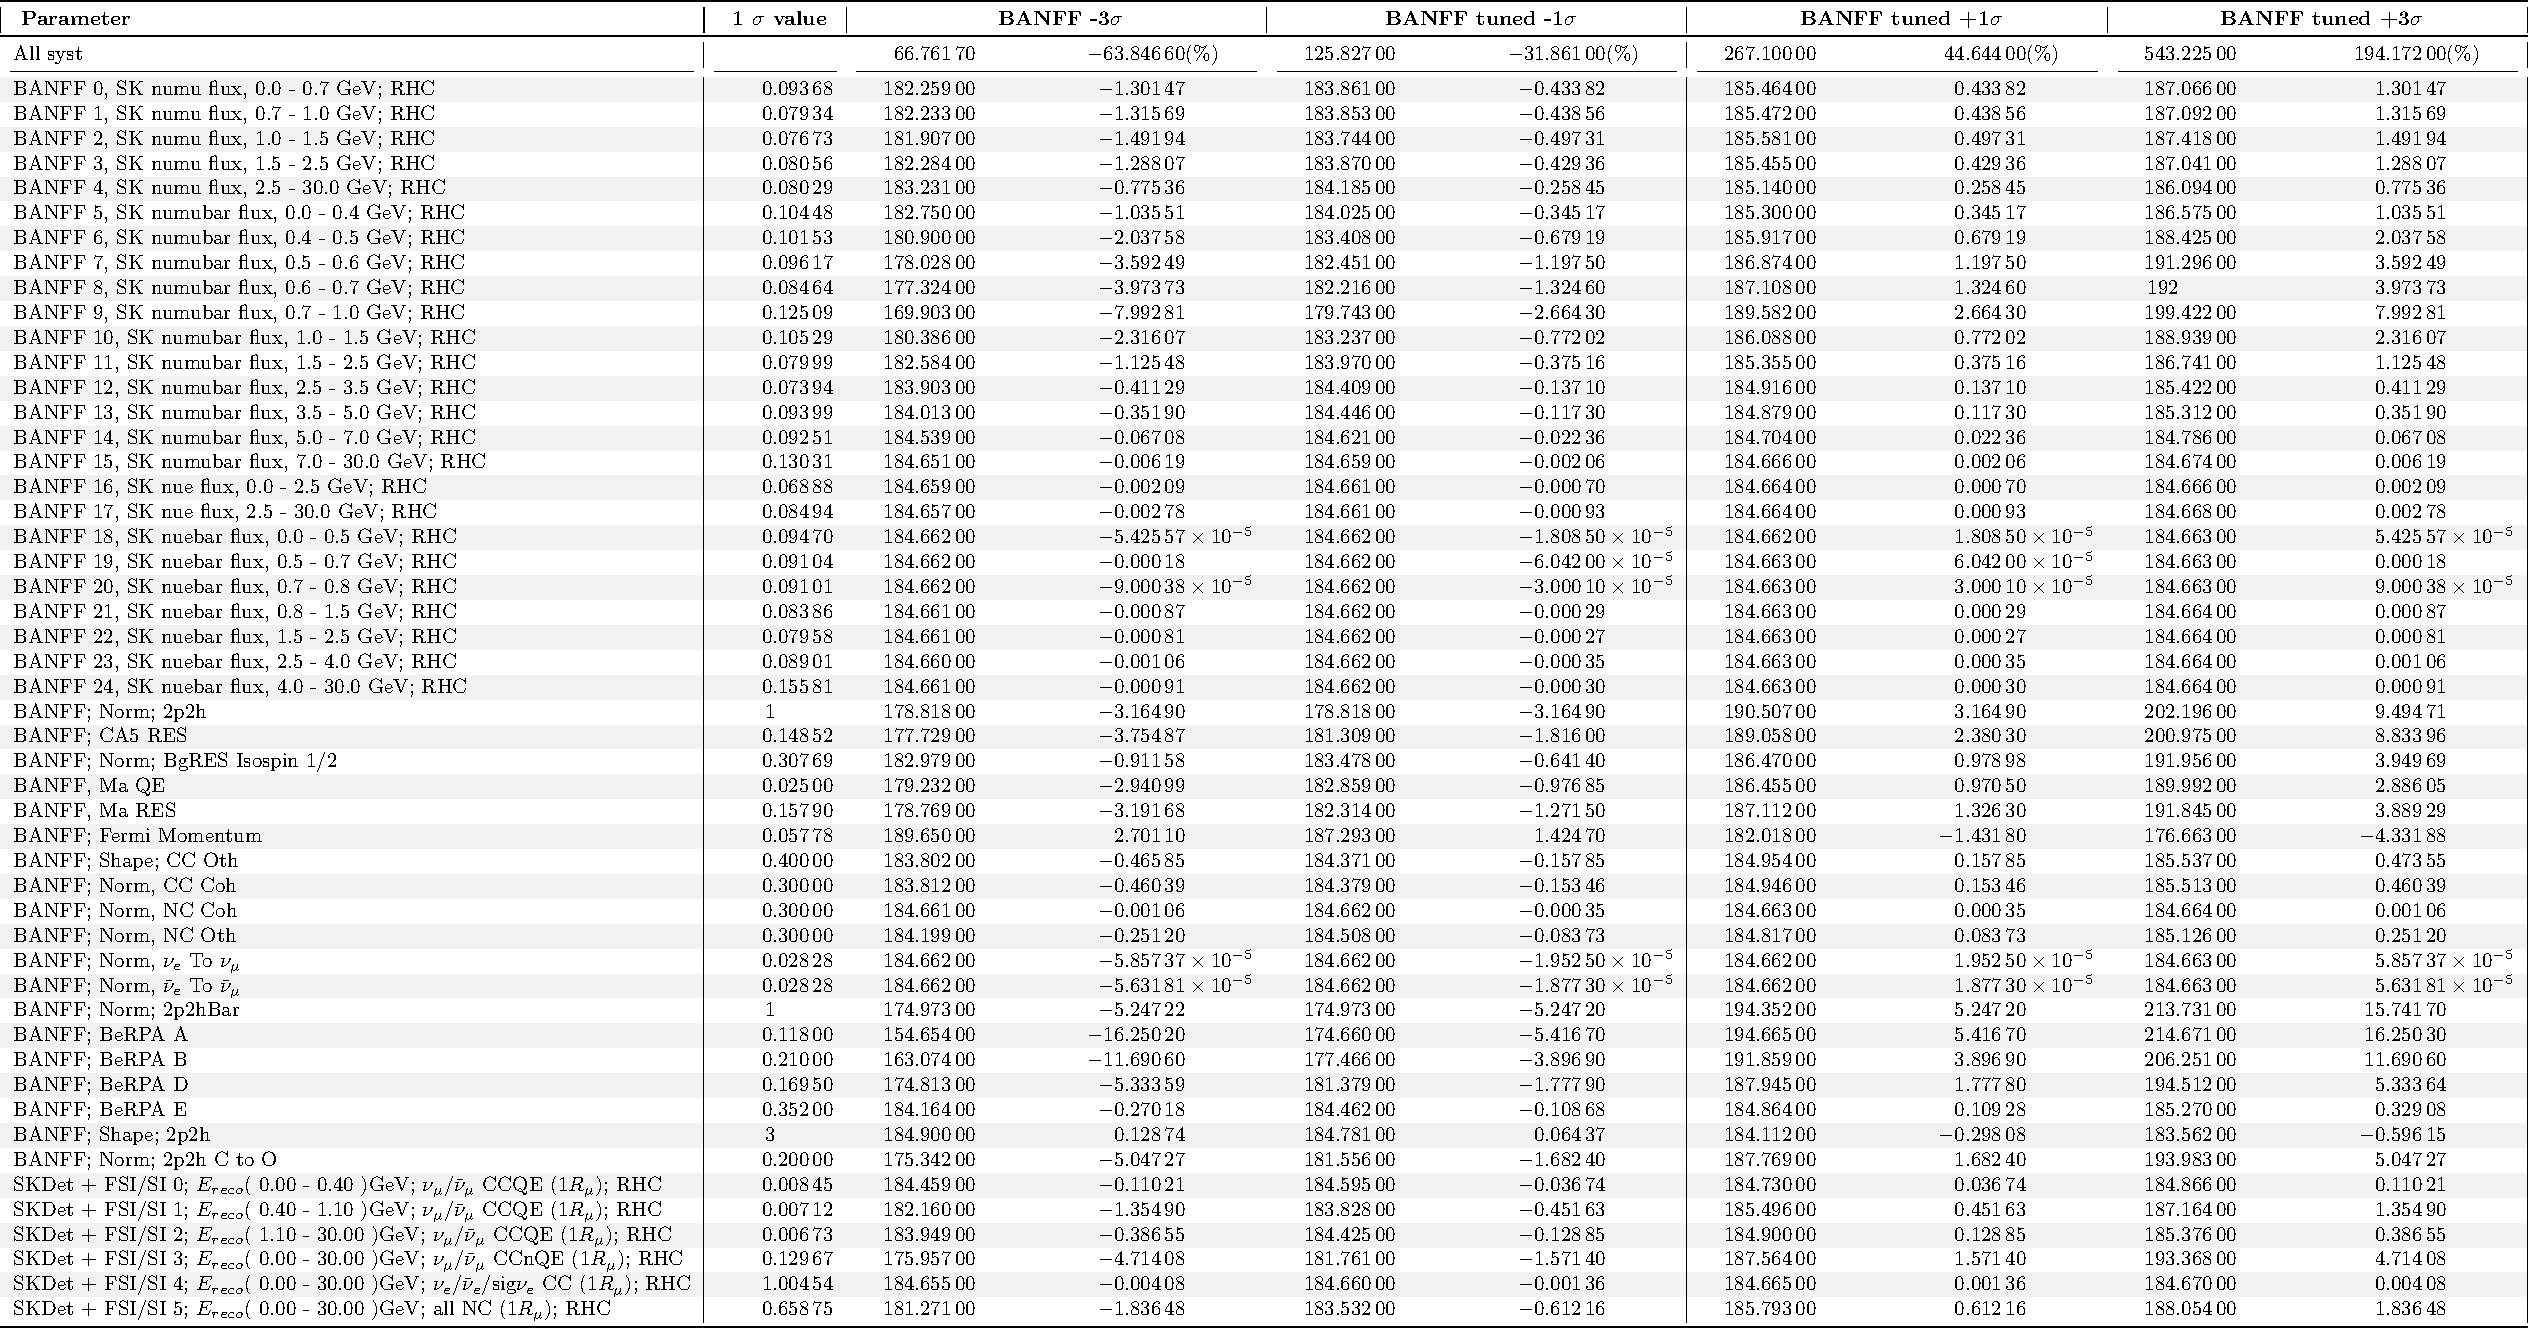
\includegraphics[page=1, trim={0cm 0cm 0cm 0cm}, clip, scale=0.25] {images/variations/tables/systematic_tables_prefit_unosc_RHC1Rmu}
	\end{figure}
\end{frame}

\begin{frame}{RHC $e$-like pre-BANFF unoscillated}
	\centering
	\begin{figure}
		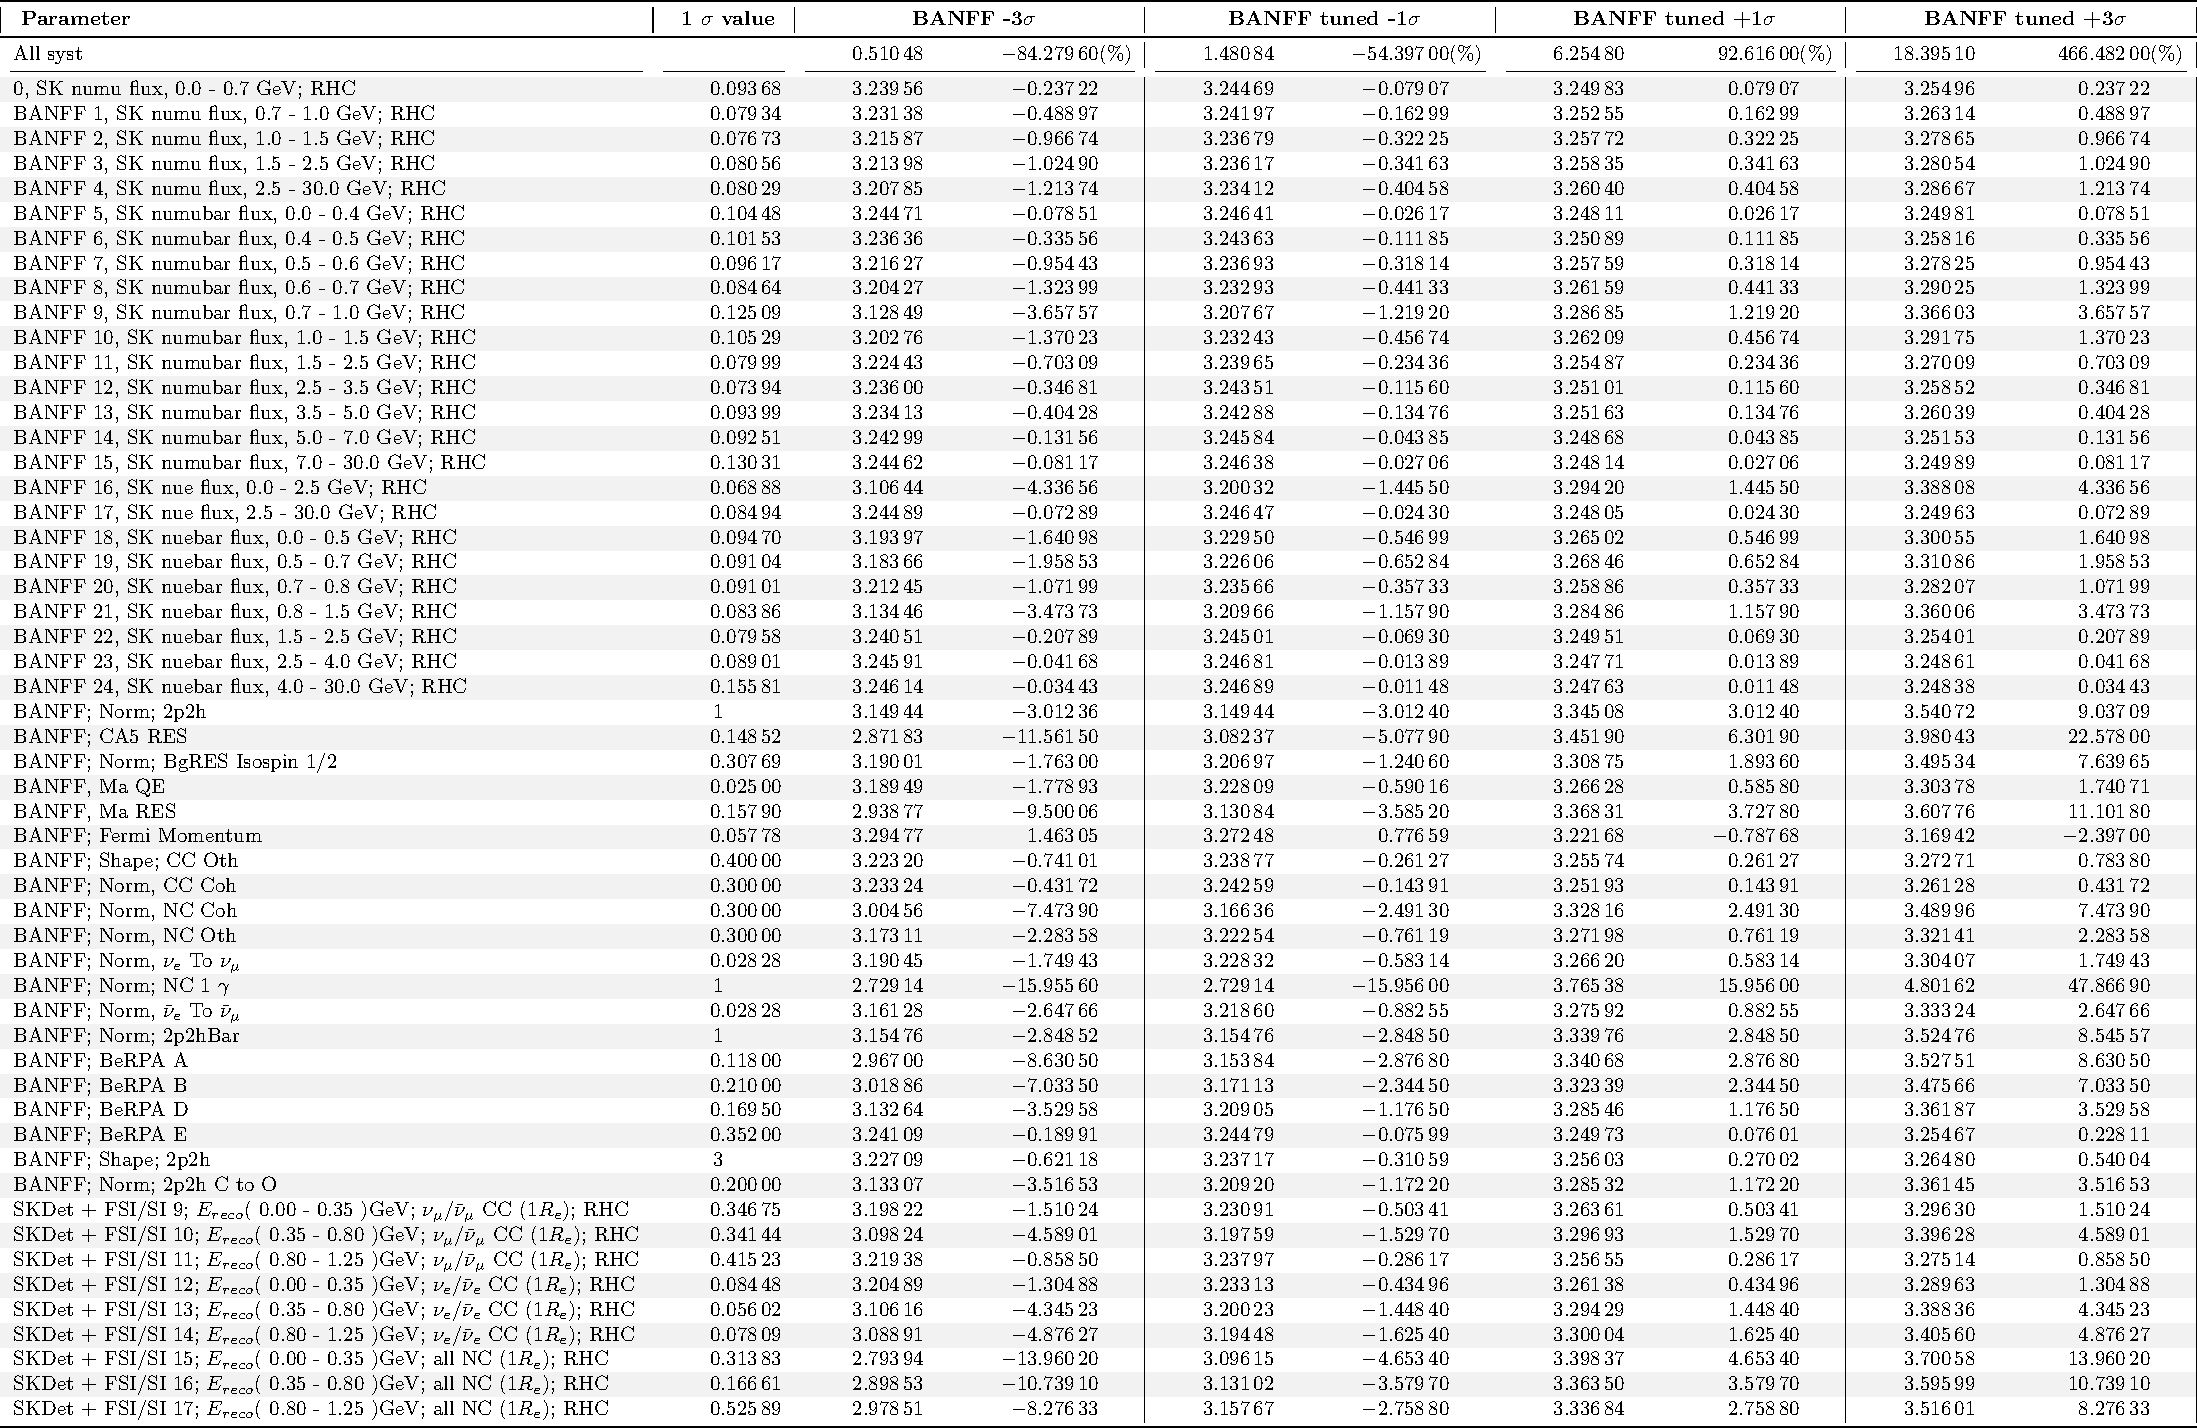
\includegraphics[page=1, trim={0cm 0cm 0cm 0cm}, clip, scale=0.3] {images/variations/tables/systematic_tables_prefit_unosc_RHC1Re}
	\end{figure}
\end{frame}

\end{document}

